% Options for packages loaded elsewhere
\PassOptionsToPackage{unicode}{hyperref}
\PassOptionsToPackage{hyphens}{url}
%
\documentclass[
]{article}
\usepackage{amsmath,amssymb}
\usepackage{lmodern}
\usepackage{iftex}
\ifPDFTeX
  \usepackage[T1]{fontenc}
  \usepackage[utf8]{inputenc}
  \usepackage{textcomp} % provide euro and other symbols
\else % if luatex or xetex
  \usepackage{unicode-math}
  \defaultfontfeatures{Scale=MatchLowercase}
  \defaultfontfeatures[\rmfamily]{Ligatures=TeX,Scale=1}
\fi
% Use upquote if available, for straight quotes in verbatim environments
\IfFileExists{upquote.sty}{\usepackage{upquote}}{}
\IfFileExists{microtype.sty}{% use microtype if available
  \usepackage[]{microtype}
  \UseMicrotypeSet[protrusion]{basicmath} % disable protrusion for tt fonts
}{}
\makeatletter
\@ifundefined{KOMAClassName}{% if non-KOMA class
  \IfFileExists{parskip.sty}{%
    \usepackage{parskip}
  }{% else
    \setlength{\parindent}{0pt}
    \setlength{\parskip}{6pt plus 2pt minus 1pt}}
}{% if KOMA class
  \KOMAoptions{parskip=half}}
\makeatother
\usepackage{xcolor}
\IfFileExists{xurl.sty}{\usepackage{xurl}}{} % add URL line breaks if available
\IfFileExists{bookmark.sty}{\usepackage{bookmark}}{\usepackage{hyperref}}
\hypersetup{
  pdftitle={Exploring the transmission advantage of Omicron in England},
  pdfauthor={Epiforecasts},
  hidelinks,
  pdfcreator={LaTeX via pandoc}}
\urlstyle{same} % disable monospaced font for URLs
\usepackage[margin=1in]{geometry}
\usepackage{longtable,booktabs,array}
\usepackage{calc} % for calculating minipage widths
% Correct order of tables after \paragraph or \subparagraph
\usepackage{etoolbox}
\makeatletter
\patchcmd\longtable{\par}{\if@noskipsec\mbox{}\fi\par}{}{}
\makeatother
% Allow footnotes in longtable head/foot
\IfFileExists{footnotehyper.sty}{\usepackage{footnotehyper}}{\usepackage{footnote}}
\makesavenoteenv{longtable}
\usepackage{graphicx}
\makeatletter
\def\maxwidth{\ifdim\Gin@nat@width>\linewidth\linewidth\else\Gin@nat@width\fi}
\def\maxheight{\ifdim\Gin@nat@height>\textheight\textheight\else\Gin@nat@height\fi}
\makeatother
% Scale images if necessary, so that they will not overflow the page
% margins by default, and it is still possible to overwrite the defaults
% using explicit options in \includegraphics[width, height, ...]{}
\setkeys{Gin}{width=\maxwidth,height=\maxheight,keepaspectratio}
% Set default figure placement to htbp
\makeatletter
\def\fps@figure{htbp}
\makeatother
\setlength{\emergencystretch}{3em} % prevent overfull lines
\providecommand{\tightlist}{%
  \setlength{\itemsep}{0pt}\setlength{\parskip}{0pt}}
\setcounter{secnumdepth}{5}
\ifLuaTeX
  \usepackage{selnolig}  % disable illegal ligatures
\fi

\title{Exploring the transmission advantage of Omicron in England}
\author{Epiforecasts}
\date{16 December 2021}

\begin{document}
\maketitle

\hypertarget{aims}{%
\subsubsection*{Aims}\label{aims}}
\addcontentsline{toc}{subsubsection}{Aims}

\begin{itemize}
\tightlist
\item
  We aimed to assess competing explanations of the transmission advantage of Omicron, compared to the existing dominant strain, Delta, in England.
\item
  We explored the likelihood of increased transmissibility compared to immune escape, using S-gene target failure as a proxy for infection with Omicron.
\item
  We use a model framework where we vary only the relationship between variants while holding all other parameters constant.
\end{itemize}

\hypertarget{methods}{%
\subsubsection*{Methods}\label{methods}}
\addcontentsline{toc}{subsubsection}{Methods}

\begin{itemize}
\tightlist
\item
  Data are all test-positive cases for England. Omicron is modelled from those cases reporting an S-gene target result (failure or positive).
\item
  We used raw (unsmoothed) data by onset date (figure \ref{fig:plot-raw-data}).
\item
  Models are based on data between 2021-11-21 and 2021-12-09. We used only the most recent three weeks of data and excluded the latest 3 reported data.
\item
  We modelled at a 1 day resolution with a 7 day forecast.
\item
  We used a weakly informative prior for a transmission advantage for the VoC vs non-VoC cases of mean 0.21 (standard deviation 0.2), based on early work from South Africa\footnote{2021-12-03, Carl Pearson and others, ``Omicron spread in South Africa'', Epidemics8}
\item
  We defined the relationship between variants as scaled and correlated.
\end{itemize}

\hypertarget{results}{%
\subsubsection*{Results}\label{results}}
\addcontentsline{toc}{subsubsection}{Results}

\begin{figure}
\centering
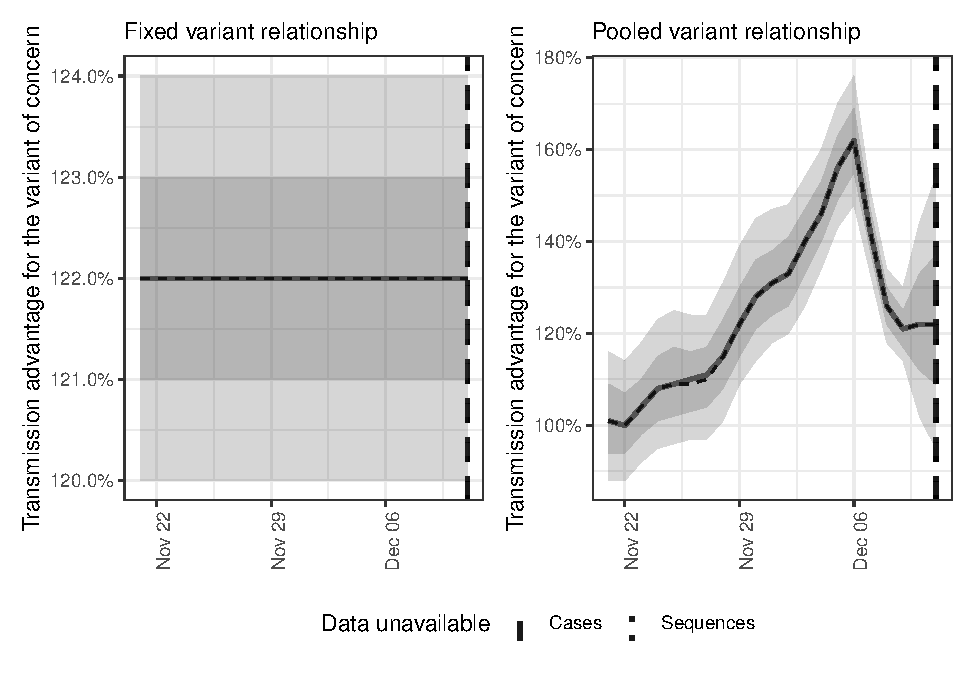
\includegraphics{transmission-results_files/figure-latex/plot-voc-advantage-1.pdf}
\caption{\label{fig:plot-voc-advantage}The transmission advantage of Omicron, modelled in a fixed relationship to Delta (left) and a time-varying relationship (right).}
\end{figure}

Transmission advantage is shown where 100\% is equivalent to the current dominant strain, Delta (figure \ref{fig:plot-voc-advantage}). Both models indicated a stronger transmission advantage for Omicron.

\begin{itemize}
\tightlist
\item
  In a fixed relationship estimated Omicron advantage is 1.37 (95\% credible interval 1.35 - 1.39).
\item
  In an correlated relationship Omicron advantage is 1.33 (95\% CrI 1.22 - 1.45).
\item
  We estimated the growth rate (figure \ref{fig:plot-growth-rt}), the proportion of cases attributable to Omicron (figure \ref{fig:plot-voc-frac}) and case counts (figure \ref{fig:plot-cases}).
\end{itemize}

\begin{figure}
\centering
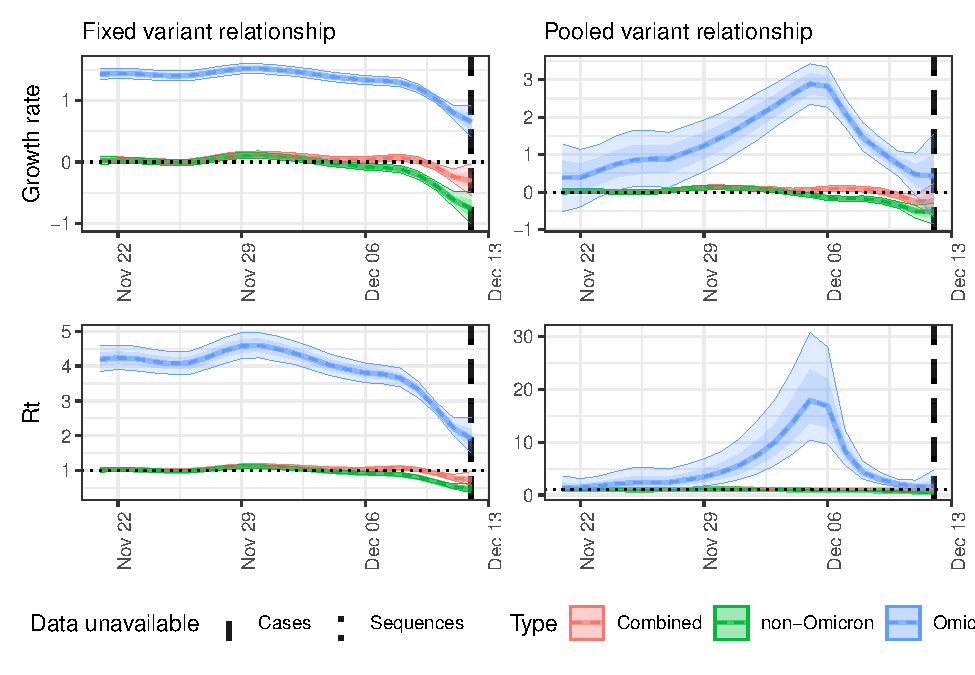
\includegraphics{transmission-results_files/figure-latex/plot-growth-rt-1.pdf}
\caption{\label{fig:plot-growth-rt}The growth rate and reproduction number of Omicron, modelled in a fixed relationship to Delta (left) and a time-varying relationship (right).}
\end{figure}

\begin{figure}
\centering
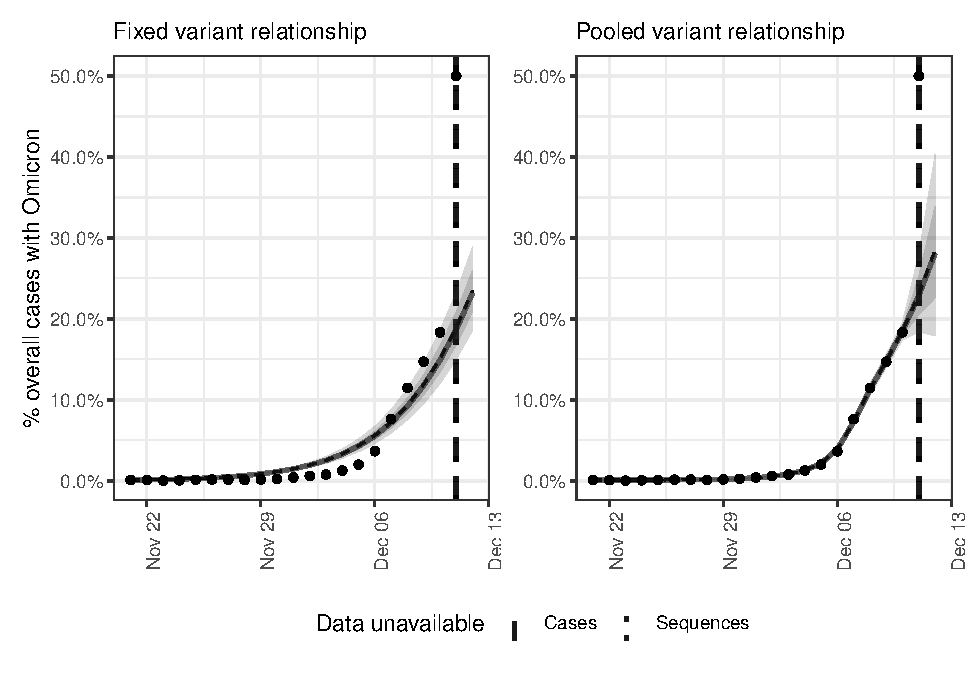
\includegraphics{transmission-results_files/figure-latex/plot-voc-frac-1.pdf}
\caption{\label{fig:plot-voc-frac}Fraction of cases attributable to Omicron, modelled in a fixed relationship to Delta (left) and a time-varying relationship (right).}
\end{figure}

\begin{figure}
\centering
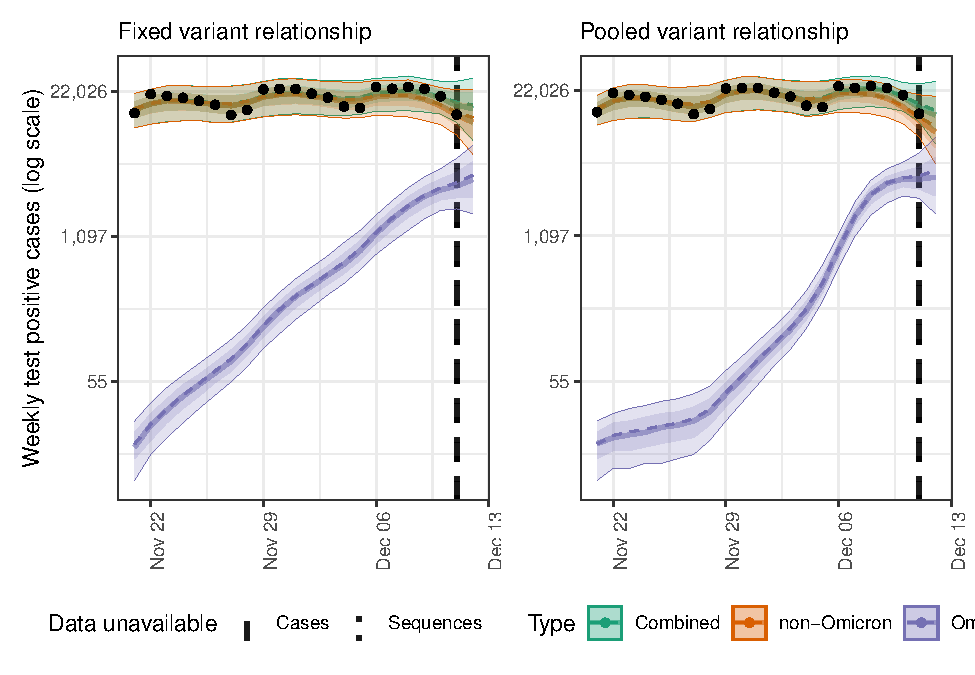
\includegraphics{transmission-results_files/figure-latex/plot-cases-1.pdf}
\caption{\label{fig:plot-cases}Weekly cases shown on a log scale, modelled in a fixed relationship to Delta (left) and a time-varying relationship (right).}
\end{figure}

\hypertarget{model-comparison}{%
\paragraph*{Model comparison}\label{model-comparison}}
\addcontentsline{toc}{paragraph}{Model comparison}

\begin{itemize}
\tightlist
\item
  Comparing the models on PSIS-LOO indicated an estimated difference in expected log pointwise predictive density of -3.29 (with a standard error of 1.32) for the correlated model compared to the scaled model.
\item
  We also compared each model using model scoring.
\end{itemize}

\begin{tabular}{l|r|r|r|r|r|r}
\hline
Variant relationship & interval\_score & sharpness & underprediction & overprediction & coverage\_deviation & bias\\
\hline
scaled & 858 & 733 & 94 & 32 & 0.12 & -0.18\\
\hline
correlated & 857 & 733 & 91 & 33 & 0.14 & -0.45\\
\hline
\end{tabular}
\newpage

\hypertarget{raw-data}{%
\subsubsection*{Raw data}\label{raw-data}}
\addcontentsline{toc}{subsubsection}{Raw data}

\begin{figure}
\centering
\includegraphics{transmission-results_files/figure-latex/plot-raw-data-1.pdf}
\caption{\label{fig:plot-raw-data}Raw data}
\end{figure}

\end{document}
